\tikzset{%
  every neuron/.style={
    circle,
    draw,
    minimum size=0.5cm
  },
  neuron missing/.style={
    draw=none, 
    scale=3,
    text height=0.333cm,
    execute at begin node=\color{black}$\vdots$
  },
  rect neuron/.style={ % Define the style for rectangle nodes
  rectangle,
  draw,
  minimum size=0.5cm,
  align=center, 
  },
  cross/.style={
    path picture={
      \draw[black]
        (path picture bounding box.south east) -- (path picture bounding box.north west)
        (path picture bounding box.south west) -- (path picture bounding box.north east);
    }
  },
}

\begin{figure}[ht]
\centering
    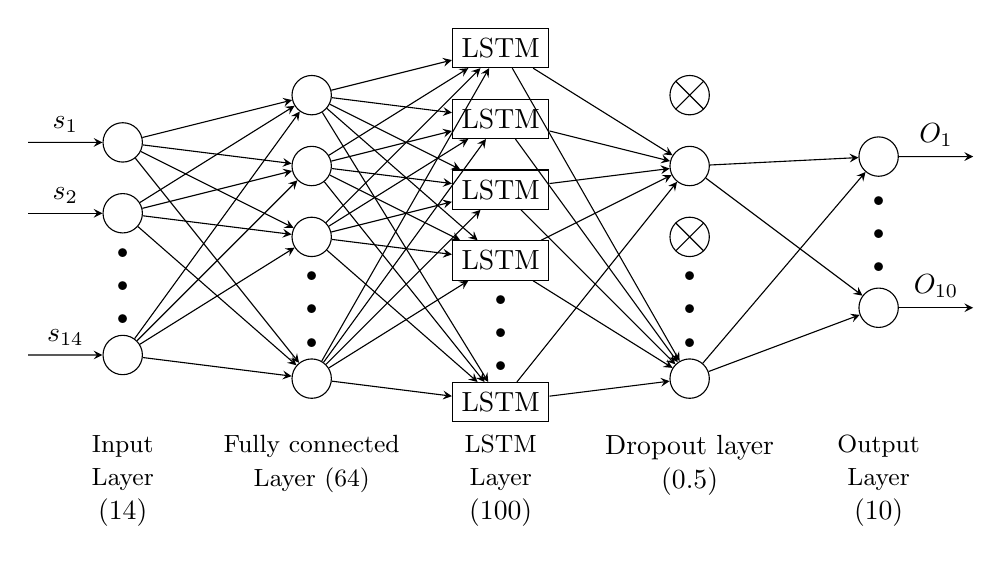
\begin{tikzpicture}[x=1.5cm, y=1.5cm, >=stealth, auto, scale=0.8]
        \foreach \m/\l [count=\y] in {1,2,missing,3}
          \node [every neuron/.try, neuron \m/.try] (input-\m) at (0,2-\y*.75) {};
        \foreach \m [count=\y] in {1,2,3,missing,4}
          \node [every neuron/.try, neuron \m/.try ] (hidden1-\m) at (2,2.5-\y*0.75) {};
        \node [rect neuron/.try, neuron 1/.try] (hidden2-1) at (4,3-1*0.75) {LSTM};
        \node [rect neuron/.try, neuron 2/.try] (hidden2-2) at (4,3-2*0.75) {LSTM};
        \node [rect neuron/.try, neuron 3/.try] (hidden2-3) at (4,3-3*0.75) {LSTM};
        \node [rect neuron/.try, neuron 4/.try] (hidden2-4) at (4,3-4*0.75) {LSTM};
        \node [rect neuron/.try, neuron missing/.try] (hidden2-missing) at (4,3-5*0.75) {};
        \node [rect neuron/.try, neuron 5/.try] (hidden2-5) at (4,3-6*0.75) {LSTM};

        % Dropout Layer
        \node [every neuron/.try, neuron 1/.try ] (dropout-1) at (6,2.5-2*0.75) {};
        \node [every neuron/.try, neuron missing/.try ] (dropout-missing) at (6,2.5-4*0.75) {};
        \node [every neuron/.try, neuron 1/.try ] (dropout-2) at (6,2.5-5*0.75) {};
        \node [every neuron/.try, neuron 1/.try, cross] (dropouted-1) at (6,2.5-1*0.75) {};
        \node [every neuron/.try, neuron 1/.try, cross] (dropouted-2) at (6,2.5-3*0.75) {};
        \foreach \m [count=\y] in {1,missing,2}
          \node [every neuron/.try, neuron \m/.try] (output-\m) at (8,1.9-\y*.8) {};
        \foreach \l [count=\i] in {1,2,14}
          \draw [<-] (input-\i) -- ++(-1,0)
            node [above, midway] {$s_{\l}$};
        \foreach \l [count=\i] in {1,10}
          \draw [->] (output-\i) -- ++(1,0)
            node [above, midway] {$O_{\l}$};
    
        \foreach \i in {1,...,3}
          \foreach \j in {1,...,4}
            \draw [->] (input-\i) -- (hidden1-\j);
        \foreach \i in {1,...,4}
          \foreach \j in {1,...,5}
            \draw [->] (hidden1-\i) -- (hidden2-\j);
        \foreach \i in {1,...,5}
          \foreach \j in {1,...,2}
            \draw [->] (hidden2-\i) -- (dropout-\j);
        \foreach \i in {1,...,2}
          \foreach \j in {1,...,2}
            \draw [->] (dropout-\i) -- (output-\j);
        \foreach \l [count=\x from 0] in {\small Input \\\small Layer\\(14), \small Fully connected \\\small Layer (64), \small LSTM \\\small Layer \\(100), Dropout layer \\(0.5), \small Output \\\small Layer\\(10)}
          \node [align=center, below, yshift=-4.5cm] at (\x*2,2) {\l};
    \end{tikzpicture}
    \caption{\ac{LSTM} \ac{RNN} Architecture. The figure illustrates the architecture of an LSTM-based  RNN. The initial layer comprises the input data, followed by a fully connected layer featuring 64 neurons. Subsequently, the fully connected layer is seamlessly activated by a \ac{ReLU} function before connected to a bidirectional LSTM layer with 100 hidden units. A Dropout layer with 0.5 probability is strategically incorporated before the output layers. }
    \label{fig:lstmstruct}
\end{figure}
        % \foreach \l [count=\i] in {1,2,3,64}
        %   \node [above] at (hidden1-\i.north) {$H_{1,\l}$};
        % \foreach \l [count=\i] in {1,2,3,4,128}
        %   \node [above] at (hidden2-\i.north) {$H_{2,\l}$};
        % \foreach \l [count=\i] in {1,2,3,64}
        %   \node [above] at (hidden3-\i.north) {$H_{3,\l}$};